% !TeX encoding = UTF-8
% !TeX program = xelatex
% !TeX spellcheck = en_US

\documentclass[degree=master]{thuthesis}
  % 学位 degree:
  %   doctor | master | bachelor | postdoc
  % 学位类型 degree-type:
  %   academic(默认)| professional
  % 语言 language
  %   chinese(默认)| english
  % 字体库 fontset
  %   windows | mac | fandol | ubuntu
  % 建议终版使用 Windows 平台的字体编译


% 论文基本配置,加载宏包等全局配置
% !TeX root = ./thuthesis-example.tex

% 论文基本信息配置

\thusetup{
  %******************************
  % 注意:
  %   1. 配置里面不要出现空行
  %   2. 不需要的配置信息可以删除
  %   3. 建议先阅读文档中所有关于选项的说明
  %******************************
  %
  % 输出格式
  %   选择打印版(print)或用于提交的电子版(electronic),前者会插入空白页以便直接双面打印
  %
  output = print,
  %
  % 标题
  %   可使用“\\”命令手动控制换行
  %
  title  = {清华大学学位论文 \LaTeX{} 模板\\使用示例文档 v\version},
  title* = {An Introduction to \LaTeX{} Thesis Template of Tsinghua
            University v\version},
  %
  % 学位
  %   1. 学术型
  %      - 中文
  %        需注明所属的学科门类,例如:
  %        哲学、经济学、法学、教育学、文学、历史学、理学、工学、农学、医学、
  %        军事学、管理学、艺术学
  %      - 英文
  %        博士:Doctor of Philosophy
  %        硕士:
  %          哲学、文学、历史学、法学、教育学、艺术学门类,公共管理学科
  %          填写“Master of Arts“,其它填写“Master of Science”
  %   2. 专业型
  %      直接填写专业学位的名称,例如:
  %      教育博士、工程硕士等
  %      Doctor of Education, Master of Engineering
  %   3. 本科生不需要填写
  %
  degree-name  = {工学硕士},
  degree-name* = {Master of Science},
  %
  % 培养单位
  %   填写所属院系的全名
  %
  department = {计算机科学与技术系},
  %
  % 学科
  %   1. 学术型学位
  %      获得一级学科授权的学科填写一级学科名称,其他填写二级学科名称
  %   2. 工程硕士
  %      工程领域名称
  %   3. 其他专业型学位
  %      不填写此项
  %   4. 本科生填写专业名称,第二学位论文需标注“(第二学位)”
  %
  discipline  = {计算机科学与技术},
  discipline* = {Computer Science and Technology},
  %
  % 姓名
  %
  author  = {薛瑞尼},
  author* = {Xue Ruini},
  %
  % 指导教师
  %   中文姓名和职称之间以英文逗号“,”分开,下同
  %
  supervisor  = {郑纬民, 教授},
  supervisor* = {Professor Zheng Weimin},
  %
  % 副指导教师
  %
  associate-supervisor  = {陈文光, 教授},
  associate-supervisor* = {Professor Chen Wenguang},
  %
  % 联合指导教师
  %
  % co-supervisor  = {某某某, 教授},
  % co-supervisor* = {Professor Mou Moumou},
  %
  % 日期
  %   使用 ISO 格式;默认为当前时间
  %
  % date = {2019-07-07},
  %
  % 是否在中文封面后的空白页生成书脊(默认 false)
  %
  include-spine = false,
  %
  % 密级和年限
  %   秘密, 机密, 绝密
  %
  % secret-level = {秘密},
  % secret-year  = {10},
  %
  % 博士后专有部分
  %
  % clc                = {分类号},
  % udc                = {UDC},
  % id                 = {编号},
  % discipline-level-1 = {计算机科学与技术},  % 流动站(一级学科)名称
  % discipline-level-2 = {系统结构},          % 专业(二级学科)名称
  % start-date         = {2011-07-01},        % 研究工作起始时间
}

% 载入所需的宏包

% 定理类环境宏包
\usepackage{amsthm}
% 也可以使用 ntheorem
% \usepackage[amsmath,thmmarks,hyperref]{ntheorem}

\thusetup{
  %
  % 数学字体
  % math-style = GB,  % GB | ISO | TeX
  math-font  = xits,  % sitx | xits | libertinus
}

% 可以使用 nomencl 生成符号和缩略语说明
% \usepackage{nomencl}
% \makenomenclature

% 表格加脚注
\usepackage{threeparttable}

% 表格中支持跨行
\usepackage{multirow}

% 固定宽度的表格。
% \usepackage{tabularx}

% 跨页表格
\usepackage{longtable}

% 算法
\usepackage{algorithm}
\usepackage{algorithmic}

% 量和单位
\usepackage{siunitx}

% 参考文献使用 BibTeX + natbib 宏包
% 顺序编码制
\usepackage[sort]{natbib}
\bibliographystyle{thuthesis-numeric}

% 著者-出版年制
% \usepackage{natbib}
% \bibliographystyle{thuthesis-author-year}

% 本科生参考文献的著录格式
% \usepackage[sort]{natbib}
% \bibliographystyle{thuthesis-bachelor}

% 参考文献使用 BibLaTeX 宏包
% \usepackage[style=thuthesis-numeric]{biblatex}
% \usepackage[style=thuthesis-author-year]{biblatex}
% \usepackage[style=apa]{biblatex}
% \usepackage[style=mla-new]{biblatex}
% 声明 BibLaTeX 的数据库
% \addbibresource{ref/refs.bib}

% 定义所有的图片文件在 figures 子目录下
\graphicspath{{figures/}}

% 数学命令
\makeatletter
\newcommand\dif{%  % 微分符号
  \mathop{}\!%
  \ifthu@math@style@TeX
    d%
  \else
    \mathrm{d}%
  \fi
}
\makeatother

% hyperref 宏包在最后调用
\usepackage{hyperref}



\begin{document}

% 封面
% \maketitle

% 学位论文指导小组、公开评阅人和答辩委员会名单
% 本科生不需要
% % % !TeX root = ../thuthesis-example.tex

% \begin{committee}[name={学位论文指导小组、公开评阅人和答辩委员会名单}]

%   \newcolumntype{C}[1]{@{}>{\centering\arraybackslash}p{#1}}

%   \section*{指导小组名单}

%   \begin{center}
%     \begin{tabular}{C{3cm}C{3cm}C{9cm}@{}}
%       李XX & 教授     & 清华大学 \\
%       王XX & 副教授   & 清华大学 \\
%       张XX & 助理教授 & 清华大学 \\
%     \end{tabular}
%   \end{center}


%   \section*{公开评阅人名单}

%   \begin{center}
%     \begin{tabular}{C{3cm}C{3cm}C{9cm}@{}}
%       刘XX & 教授   & 清华大学                    \\
%       陈XX & 副教授 & XXXX大学                    \\
%       杨XX & 研究员 & 中国XXXX科学院XXXXXXX研究所 \\
%     \end{tabular}
%   \end{center}


%   \section*{答辩委员会名单}

%   \begin{center}
%     \begin{tabular}{C{2.75cm}C{2.98cm}C{4.63cm}C{4.63cm}@{}}
%       主席 & 赵XX                  & 教授                    & 清华大学       \\
%       委员 & 刘XX                  & 教授                    & 清华大学       \\
%           & \multirow{2}{*}{杨XX} & \multirow{2}{*}{研究员} & 中国XXXX科学院 \\
%           &                       &                         & XXXXXXX研究所  \\
%           & 黄XX                  & 教授                    & XXXX大学       \\
%           & 周XX                  & 副教授                  & XXXX大学       \\
%       秘书 & 吴XX                  & 助理研究员              & 清华大学       \\
%     \end{tabular}
%   \end{center}

% \end{committee}



% % 也可以导入 Word 版转的 PDF 文件
% % \begin{committee}[file=figures/committee.pdf]
% % \end{committee}


% 使用授权的说明
% \copyrightpage
% 将签字扫描后授权文件 scan-copyright.pdf 替换原始页面
% \copyrightpage[file=scan-copyright.pdf]

\frontmatter
% !TeX root = ../thuthesis-example.tex

% 中英文摘要和关键字

\begin{abstract}
  论文的摘要是对论文研究内容和成果的高度概括。
  摘要应对论文所研究的问题及其研究目的进行描述,对研究方法和过程进行简单介绍,对研究成果和所得结论进行概括。
  摘要应具有独立性和自明性,其内容应包含与论文全文同等量的主要信息。
  使读者即使不阅读全文,通过摘要就能了解论文的总体内容和主要成果。

  论文摘要的书写应力求精确、简明。
  切忌写成对论文书写内容进行提要的形式,尤其要避免“第 1 章……;第 2 章……;……”这种或类似的陈述方式。

  关键词是为了文献标引工作、用以表示全文主要内容信息的单词或术语。
  关键词不超过 5 个,每个关键词中间用分号分隔。

  % 关键词用“英文逗号”分隔,输出时会自动处理为正确的分隔符
  \thusetup{
    keywords = {关键词 1, 关键词 2, 关键词 3, 关键词 4, 关键词 5},
  }
\end{abstract}

\begin{abstract*}
  An abstract of a dissertation is a summary and extraction of research work and contributions.
  Included in an abstract should be description of research topic and research objective, brief introduction to methodology and research process, and summary of conclusion and contributions of the research.
  An abstract should be characterized by independence and clarity and carry identical information with the dissertation.
  It should be such that the general idea and major contributions of the dissertation are conveyed without reading the dissertation.

  An abstract should be concise and to the point.
  It is a misunderstanding to make an abstract an outline of the dissertation and words “the first chapter”, “the second chapter” and the like should be avoided in the abstract.

  Keywords are terms used in a dissertation for indexing, reflecting core information of the dissertation.
  An abstract may contain a maximum of 5 keywords, with semi-colons used in between to separate one another.

  % Use comma as separator when inputting
  \thusetup{
    keywords* = {keyword 1, keyword 2, keyword 3, keyword 4, keyword 5},
  }
\end{abstract*}


% 目录
\tableofcontents

% 插图和附表清单
% 本科生的插图索引和表格索引需要移至正文之后、参考文献前
% \listoffiguresandtables  % 插图和附表清单(仅限研究生)
% \listoffigures           % 插图清单
% \listoftables            % 附表清单

% 符号对照表
% % !TeX root = ../thuthesis-example.tex

\begin{denotation}[3cm]
  \item[PI] 聚酰亚胺
  \item[MPI] 聚酰亚胺模型化合物,N-苯基邻苯酰亚胺
  \item[PBI] 聚苯并咪唑
  \item[MPBI] 聚苯并咪唑模型化合物,N-苯基苯并咪唑
  \item[PY] 聚吡咙
  \item[PMDA-BDA] 均苯四酸二酐与联苯四胺合成的聚吡咙薄膜
  \item[MPY] 聚吡咙模型化合物
  \item[As-PPT] 聚苯基不对称三嗪
  \item[MAsPPT] 聚苯基不对称三嗪单模型化合物,3,5,6-三苯基-1,2,4-三嗪
  \item[DMAsPPT] 聚苯基不对称三嗪双模型化合物(水解实验模型化合物)
  \item[S-PPT] 聚苯基对称三嗪
  \item[MSPPT] 聚苯基对称三嗪模型化合物,2,4,6-三苯基-1,3,5-三嗪
  \item[PPQ] 聚苯基喹噁啉
  \item[MPPQ] 聚苯基喹噁啉模型化合物,3,4-二苯基苯并二嗪
  \item[HMPI] 聚酰亚胺模型化合物的质子化产物
  \item[HMPY] 聚吡咙模型化合物的质子化产物
  \item[HMPBI] 聚苯并咪唑模型化合物的质子化产物
  \item[HMAsPPT] 聚苯基不对称三嗪模型化合物的质子化产物
  \item[HMSPPT] 聚苯基对称三嗪模型化合物的质子化产物
  \item[HMPPQ] 聚苯基喹噁啉模型化合物的质子化产物
  \item[PDT] 热分解温度
  \item[HPLC] 高效液相色谱(High Performance Liquid Chromatography)
  \item[HPCE] 高效毛细管电泳色谱(High Performance Capillary lectrophoresis)
  \item[LC-MS] 液相色谱-质谱联用(Liquid chromatography-Mass Spectrum)
  \item[TIC] 总离子浓度(Total Ion Content)
  \item[\textit{ab initio}] 基于第一原理的量子化学计算方法,常称从头算法
  \item[DFT] 密度泛函理论(Density Functional Theory)
  \item[$E_a$] 化学反应的活化能(Activation Energy)
  \item[ZPE] 零点振动能(Zero Vibration Energy)
  \item[PES] 势能面(Potential Energy Surface)
  \item[TS] 过渡态(Transition State)
  \item[TST] 过渡态理论(Transition State Theory)
  \item[$\increment G^\neq$] 活化自由能(Activation Free Energy)
  \item[$\kappa$] 传输系数(Transmission Coefficient)
  \item[IRC] 内禀反应坐标(Intrinsic Reaction Coordinates)
  \item[$\nu_i$] 虚频(Imaginary Frequency)
  \item[ONIOM] 分层算法(Our own N-layered Integrated molecular Orbital and molecular Mechanics)
  \item[SCF] 自洽场(Self-Consistent Field)
  \item[SCRF] 自洽反应场(Self-Consistent Reaction Field)
\end{denotation}



% 也可以使用 nomencl 宏包,需要在导言区
% \usepackage{nomencl}
% \makenomenclature

% 在这里输出符号说明
% \printnomenclature[3cm]

% 在正文中的任意为都可以标题
% \nomenclature{PI}{聚酰亚胺}
% \nomenclature{MPI}{聚酰亚胺模型化合物,N-苯基邻苯酰亚胺}
% \nomenclature{PBI}{聚苯并咪唑}
% \nomenclature{MPBI}{聚苯并咪唑模型化合物,N-苯基苯并咪唑}
% \nomenclature{PY}{聚吡咙}
% \nomenclature{PMDA-BDA}{均苯四酸二酐与联苯四胺合成的聚吡咙薄膜}
% \nomenclature{MPY}{聚吡咙模型化合物}
% \nomenclature{As-PPT}{聚苯基不对称三嗪}
% \nomenclature{MAsPPT}{聚苯基不对称三嗪单模型化合物,3,5,6-三苯基-1,2,4-三嗪}
% \nomenclature{DMAsPPT}{聚苯基不对称三嗪双模型化合物(水解实验模型化合物)}
% \nomenclature{S-PPT}{聚苯基对称三嗪}
% \nomenclature{MSPPT}{聚苯基对称三嗪模型化合物,2,4,6-三苯基-1,3,5-三嗪}
% \nomenclature{PPQ}{聚苯基喹噁啉}
% \nomenclature{MPPQ}{聚苯基喹噁啉模型化合物,3,4-二苯基苯并二嗪}
% \nomenclature{HMPI}{聚酰亚胺模型化合物的质子化产物}
% \nomenclature{HMPY}{聚吡咙模型化合物的质子化产物}
% \nomenclature{HMPBI}{聚苯并咪唑模型化合物的质子化产物}
% \nomenclature{HMAsPPT}{聚苯基不对称三嗪模型化合物的质子化产物}
% \nomenclature{HMSPPT}{聚苯基对称三嗪模型化合物的质子化产物}
% \nomenclature{HMPPQ}{聚苯基喹噁啉模型化合物的质子化产物}
% \nomenclature{PDT}{热分解温度}
% \nomenclature{HPLC}{高效液相色谱(High Performance Liquid Chromatography)}
% \nomenclature{HPCE}{高效毛细管电泳色谱(High Performance Capillary lectrophoresis)}
% \nomenclature{LC-MS}{液相色谱-质谱联用(Liquid chromatography-Mass Spectrum)}
% \nomenclature{TIC}{总离子浓度(Total Ion Content)}
% \nomenclature{\textit{ab initio}}{基于第一原理的量子化学计算方法,常称从头算法}
% \nomenclature{DFT}{密度泛函理论(Density Functional Theory)}
% \nomenclature{$E_a$}{化学反应的活化能(Activation Energy)}
% \nomenclature{ZPE}{零点振动能(Zero Vibration Energy)}
% \nomenclature{PES}{势能面(Potential Energy Surface)}
% \nomenclature{TS}{过渡态(Transition State)}
% \nomenclature{TST}{过渡态理论(Transition State Theory)}
% \nomenclature{$\increment G^\neq$}{活化自由能(Activation Free Energy)}
% \nomenclature{$\kappa$}{传输系数(Transmission Coefficient)}
% \nomenclature{IRC}{内禀反应坐标(Intrinsic Reaction Coordinates)}
% \nomenclature{$\nu_i$}{虚频(Imaginary Frequency)}
% \nomenclature{ONIOM}{分层算法(Our own N-layered Integrated molecular Orbital and molecular Mechanics)}
% \nomenclature{SCF}{自洽场(Self-Consistent Field)}
% \nomenclature{SCRF}{自洽反应场(Self-Consistent Reaction Field)}



% 正文部分
\mainmatter
% !TeX root = ../thuthesis-example.tex

\chapter{引言}

动态规划(Dynamic Programming, DP)与分治方法相似,都是通过组合子问题的解来求解原问题。分治方法将问题划分为互不相交的子问题,再将它们的解组合起来,求出原问题的解。与之相反,动态规划应用于子问题重叠的情况,即不同的子问题具有公共的子子问题(递归进行)。在这种情况下,分治算法会做许多不必要的工作,它会反复地求解那些公共子子问题。而动态规划算法对每个子子问题只求解一次,将其解保存在一个表格中,从而无需每次求解一个子子问题时都要重新计算,避免了这种不必要的计算工作。
\cite{2001Introduction}

近年来,动态规划在信息学中的应用愈发广泛。简单的动态规划模型如线性 DP、背包
DP、区间 DP
已被多数人熟练掌握并运用,本文将不再赘述。而与之形成对比的一些复杂动态规划问题由于其算法本身的难度,难以被应用或被信息学竞赛选手解答出,故本文将这些算法进行了整合并且进行了详细地解析,可以作为信息学竞赛选手及相关领域的参考资料使用。

对于一些时间复杂度本身较劣的 DP
思路,硬件运行速度的提升往往是常量级的,在数据规模快速增长时效果甚微,而直接对
DP 的状态设计进行本质优化往往具有局限性,无法系统整理并在其他 DP
上如法炮制。故本文还将介绍四种被广泛应用的 DP
转移优化方式,在保持原有状态设计和转移方式的基础上最大限度地省去不必要的计算,已达到优化时间复杂度的目的。

% !TeX root = ../thuthesis-example.tex

\chapter{基于状态压缩的动态规划}

\section{状态压缩}

状态压缩一般是将一个较小的集合内每个元素的状态通过特定的计算方法,转换为单个整数。这样的转换必须是双射。

在信息学竞赛中,状态的压缩和解压缩一般由二进制运算完成。究其主要原因,一方面是因为二进制可以很直接的表达一个元素集合内每个元素选中或不选中的状态,如二进制串
\(\mathbf{01001}\) 可以表示一个大小为 \(5\) 的集合 \(S\) 中第 \(2\) 和
\(5\) 个元素被选中,第 \(1\)、\(3\)、\(4\)
个元素未被选中的状态。另一方面,是因为计算机在存储数据时是以二进制方式存储,直接在二进制下对数据进行处理和计算往往比其他进制要快的多。

\section{位运算}

在二进制下对数据的处理和计算与数学中常用的加减乘除和逻辑运算略有不同,对整数在内存中的二进制位进行操作,就是位运算。下面是对几类位运算的定义解释和约定。

\begin{itemize}
\item
  与(\texttt{\&}):\(A\) 和 \(B\) 的按位与运算中,对 \(A\) 和 \(B\)
  二进制下的每一位的值进行数学中的逻辑与运算,得到结果中对应位的值。
\item
  或(\texttt{\textbar{}}):\(A\) 和 \(B\) 的按位或运算中,对 \(A\) 和
  \(B\)
  二进制下的每一位的值进行数学中的逻辑或运算,得到结果中对应位的值。
\item
  取反(\texttt{\textasciitilde{}}):\(A\) 的按位取反运算中,对 \(A\)
  二进制下的每一位的值进行数学中的逻辑非运算,得到结果中对应位的值。
\item
  异或(\texttt{\^{}}):\(A\) 和 \(B\) 的按位异或计算中,对 \(A\) 和
  \(B\) 二进制下的每一位的值进行如下计算:


  \begin{longtable}[]{@{}ccc@{}}
  \toprule
  A & B & A \(\oplus\) B \\
  \midrule
  \endhead
  0 & 0 & 0 \\
  0 & 1 & 1 \\
  1 & 0 & 1 \\
  1 & 1 & 0 \\
  \bottomrule
  \end{longtable}

  得到结果中对应位的值。
\item
  \(A\) 的第 \(i\) 位表示 \(A\) 在二进制下从最低往最高位数第 \(i+1\)
  位,即 \(\frac{A}{2^i}\) 除以 \(2\) 所得余数。
\item
  左移(\texttt{\textless{}\textless{}}),右移(\texttt{\textgreater{}\textgreater{}}):\texttt{x\textless{}\textless{}y}
  表示 \(x\times 2^y\),\texttt{x} 的第 \(i\) 位为
  \texttt{(x\textless{}\textless{}y)} 的第 \(i+y\)
  位,\texttt{(x\textless{}\textless{}y)} 的 \(0\sim (y-1)\) 位均为
  \(0\)。\texttt{x\textgreater{}\textgreater{}y} 表示
  \(\frac{x}{2^y}\),\texttt{x} 的第 \(i\) 位(\(i\ge y\))为
  \texttt{(x\textgreater{}\textgreater{}y)} 的第 \(i-y\) 位。
\end{itemize}

设全集为 \(\Omega\),\(|\Omega|=n\),用 \(n\) 位二进制整数 \(x\) 描述
\(\Omega\) 的一个子集 \(S\),那么 \(x\) 的第 \(i-1\) 位为 \(1\) 则表示
\(\Omega\) 中第 \(i\) 个元素属于 \(S\),为 \(0\) 则表示 \(\Omega\) 中第
\(i\) 个元素不属于
\(S\)。基于此,对于数学中对集合之间的运算和关系的命题,位运算也有对应计算方式。

\begin{itemize}

\item
  \(A\) 与 \(B\) 交集:\texttt{A\&B}。对于表示第 \(i+1\)
  个元素是否在交集中的第 \(i\) 位,该位值为 \(1\) 当且仅当 \(A\) 的第
  \(i\) 位为 \(1\) 且 \(B\) 的第 \(i\) 位为 \(1\),即 \(A\) 包含第
  \(i+1\) 个元素且 \(B\) 包含第 \(i+1\) 个元素。
\item
  \(A\) 与 \(B\) 并集:\texttt{A\textbar{}B}。对于表示第 \(i+1\)
  个元素是否在并集中的第 \(i\) 位,该位值为 \(1\) 当且仅当 \(A\) 的第
  \(i\) 位为 \(1\) 或 \(B\) 的第 \(i\) 位为 \(1\),即 \(A\) 包含第
  \(i+1\) 个元素或 \(B\) 包含第 \(i+1\) 个元素。
\item
  \(A\) 的补集:设 \texttt{O=((1\textless{}\textless{}n)-1)},这样有
  \texttt{O} 的 \(0\) 到 \(n-1\) 位均为 \(1\),则 \(A\)
  的补集为\texttt{O\^{}A}。对于表示第 \(i+1\) 个元素是否在补集中的第
  \(i\) 位,因为 \(O\) 第 \(i\) 位为 \(1\),因此该位为 \(1\) 当且仅当
  \(A\) 的第 \(i\) 位为 \(0\),即 \(A\) 不包含第 \(i+1\) 个元素。
\item
  \(A/B\):\texttt{A\^{}(A\&B)}。对于表示第 \(i+1\) 个元素是否在 \(A/B\)
  中的第 \(i\) 位,该位值为 \(1\) 当且仅当 \(A\) 第 \(i\) 位为 \(1\) 且
  \(A\cap B\) 第 \(i\) 位为 \(0\)。
\item
  \(p:\) \(A\) 是 \(B\)
  的子集:\texttt{(A\textbar{}B)==B}。若该表达式为真,那么对于第 \(i\)
  位,若 \(B\) 第 \(i\) 位为 \(0\),则 \(A\) 的第 \(i\) 位为 \(0\),若
  \(B\) 第 \(i\) 位为 \(1\),则 \(A\) 的第 \(i\) 位可取 \(0/1\)。即第
  \(i\) 个元素若不属于 \(B\),则第 \(i\) 个元素也不属于 \(A\),命题
  \(p\) 为真。
\end{itemize}

\section{适用问题类型}

为满足 DP
的无后效性,存储对应值的索引往往需要包括可以描述该阶段状态的全部信息。而对于一类需要记录整个集合内每个元素状态的问题,朴素的对某一数组指针进行中括号运算在程序中略显乏力,设计的状态往往会冗长且在转移时拖沓,因此状态压缩优化状态就成为了更优的选择。

以一类经典的 NP
问题,旅行商问题(TSP)为例,设计传统的动态规划状态需要描述每一个点是否被到达过,因此描述需要
\(n\) 维,其中 \(n\) 为点数。\(n\) 若不为常数,以动态的维数来实现 DP
的转移本身就较为困难,而就算假设 \(n\) 为常数,例如 \(6\),状态也需写成
\(f(0/1,0/1,0/1,0/1,0/1,0/1)\),转移时枚举转移前状态和转移后状态更是需要
\(7\)
个循环以上。而采取状态压缩,将每一个点是否被到达过表示为映射到的整数第
\(i\) 位是否为 \(1\),则状态只需写成 \(f(S)\),转移最少只需 \(2\)
个循环。

\section{应用实例一}

\subsection{题目来源}

题目名称:互不侵犯。

题目选自:NOI2009四川省省队选拔活动。

\subsection{题目描述}

在国际象棋中,国王能攻击它上、下、左、右、左上、左下、右上、右下八个方向上附近各一个格子,共
\(8\) 个。

现在在 \(n\times n\) 的国际象棋棋盘上摆放 \(k\)
个国王,使他们互不攻击,试求共有多少种摆放方案。

数据范围:\(1\le n\le 9,0\le k\le n\times n\).

\subsection{解题思路}

定义 \(f[i][j][S]\) 表示从第 \(1\) 行摆放到第 \(i\) 行,已经摆放了 \(j\)
个国王,第 \(i\) 行每个格子摆放状态为 \(S\) 的合法摆放方案数。其中 \(S\)
的第 \(i\) 位为 \(1\) 则表示此行从左往右数第 \(i+1\)
个格子摆放了国王,反之则没有摆放国王。

判断单行状态 \(S\) 单独出现是否合法,考虑判断
\texttt{(S\&(S\textless{}\textless{}1))==0}
是否为真。若为真则代表对于任意
\(i\),\texttt{S\&(S\textless{}\textless{}1)} 的第 \(i\) 位均为
\(0\),意味着 \(S\) 第 \(i\) 位为 \(1\) 和 \(S\) 的第 \(i-1\) 位为 \(1\)
不同时成立,即没有在同一行摆放左右相邻的国王。

判断两个状态 \(S_1\)、\(S_2\) 是否可以作为合法的相邻两行出现,考虑判断
\texttt{((S1\&S2)\textbar{}\textbar{}(S1\&(S2\textless{}\textless{}1))\textbar{}\textbar{}(S1\&(S2\textgreater{}\textgreater{}1)))==0}
是否为真。假设为假,那么如下三条至少存在一条为真

\begin{itemize}

\item
  \texttt{(S1\&S2)} 存在一位 \(i\) 使得其值为 \(1\),则 \(S_1\) 第 \(i\)
  位为 \(1\) 且 \(S_2\) 第 \(i\) 位为 \(1\),即上下相邻,不合法;
\item
  \texttt{(S1\&(S2\textless{}\textless{}1))} 存在一位 \(i\) 使得其值为
  \(1\),则 \(S_1\) 第 \(i\) 位为 \(1\) 且 \(S_2\) 第 \(i-1\) 位为
  \(1\),即互为左下和右上的关系,不合法;
\item
  \texttt{(S1\&(S2\textgreater{}\textgreater{}1))} 存在一位 \(i\)
  使得其值为 \(1\),则 \(S_1\) 第 \(i\) 位为 \(1\) 且 \(S_2\) 第 \(i+1\)
  位为 \(1\),即互为左上和右下的关系,不合法。
\end{itemize}

这三条判断和单行是否合法的判断覆盖了所有可能的不合法情况,提供了
\(\mathcal{O}(1)\) 的计算方法。而 C++ 中
\texttt{\_\_builtin\_popcount(x)} 函数可以以近似 \(\mathcal{O}(1)\)
的效率计算 \(x\) 二进制中 \(1\) 的个数,以下简写为
\(\operatorname{pc}(x)\)

转移考虑从小到大枚举 \(i\in[1,n]\),枚举 \(j\in[0,k]\),枚举合法单行状态
\(S_1\in[0,2^n)\)、\(S_2\in[0,2^n)\)。在 \(S_1\) 和 \(S_2\)
可以作为合法的相邻两行出现时,有转移 \[
f[i][j+\operatorname{pc}(S_2)][S_2]:=f[i][j+\operatorname{pc}(S_2)][S_2]+f[i-1][j][S_1]
\] 初始状态为
\(f[0][0][0]=1\),即没有填任何行时,仅在没有摆放任何国王且该行为空时存在一个方案。最终答案为
\[
Ans=\sum_{S\in[0,2^n)}f[n][k][S]
\] 即摆放了所有行,一共摆放了 \(k\)
个国王,最后一行为任意状态的合法方案总和。整体时间复杂度为
\(\mathcal{O}(nkA+2^n)\),空间复杂度为 \(\mathcal{O}(nk2^n)\),其中
\(A\) 为合法单行 \(S_1\)、\(S_2\) 组成的不同合法相邻行个数,在
\(n\le 9\) 时满足 \(A\le 683\).

\subsection{代码实现}

1.cpp

\section{应用实例二}

\subsection{题目来源}

题目名称:寿司晚宴。

题目选自:NOI2015。

\subsection{题目描述}

给定 \(n\),设全集为 \(\Omega=\{x\mid x\in[2,n]\}\).

求有多少个不同的二元组 \((A,B)\),满足:

\begin{itemize}

\item
  \(A,B\) 为 \(\Omega\) 的子集,
\item
  对于任意 \(x\in A,y\in B\),有 \(\gcd(x,y)=1\).
\end{itemize}

答案对 \(p\) 取模。

数据范围:\(2\le n\le 500\).

\subsection{解题思路}

显然不能对 \(500\) 以内的 \(95\)
个质因数进行状态压缩和转移,因为这样时空复杂度至少是
\(\mathcal{O}(2^{95})\) 的,远超一般计算机算力。

但可以发现对于任意 \(x\in[2,500]\),\(x\) 分解质因数后包含的 \(> 19\)
的质因子不会超过 \(1\) 个,\(\le19\) 的质因数仅 \(8\)
个,可以状态压缩。而我们只关注 \(\Omega\)
中每个数分解质因数后的质因子集合,因此一个数 \(i\) 可以被表示为二元组
\((p_i,S_i)\),其中 \(p_i\) 表示 \(i\) 分解质因数后 \(> 19\)
的质因子,没有则为 \(1\);\(S_i\) 表示 \(i\) 分解质因数后包含的
\(\le19\) 的质因子的集合,\(S_i\) 共 \(8\) 位,第 \(x\) 位为 \(1\)
则表示从小到大第 \(x+1\) 个质数是 \(i\) 的因子,反之则不是。

按二元组第一位给 \(n-1\) 个数分组后,可以看出除 \(p_i=1\)
的组,其余组不能即有元素属于 \(A\)、又有元素属于 \(B\)。且将 \(A\)
集合中的所有元素二元组第二位按位或后,\(B\) 集合对应值与之进行按位与应为
\(0\)。

因此可以对整体设计状态,对 \(p_i=1\) 的组合 \(p_i > 1\)
的组分别进行转移。

设 \(f[a][b]\) 表示 \(A\) 集合中所有元素第二位按位或的值为 \(a\),\(B\)
集合中所有元素第二位按位或的值为 \(b\) 且没有任意一个元素同时属于
\(A,B\),没有任意一组中即有元素属于 \(A\)、又有元素属于 \(B\) 的方案数。

\begin{itemize}
\item
  对于 \(p_i=1\) 的组,有 \[
  \begin{aligned}
  f'[a|S_i][b]&\leftarrow f[a][b]\\
  f'[a][b|S_i]&\leftarrow f[a][b]\\
  \end{aligned}
  \] 其中 \(f'\) 为新的 \(f\) 数组,在枚举完 \(a,b\) 后替换 \(f\)。即
  \(f\) 数组不是边枚举 \(a,b\) 边更新的。下同。
\item
  对于每一组,设 \(\operatorname{dp_1}[a][b]\) 为当前组没有任一元素在
  \(B\) 中的方案数, \(\operatorname{dp_2}[a][b]\)
  为当前组没有任一元素在 \(A\) 中的方案数,有 \[
  \begin{aligned}
  \operatorname{dp_1}'[a|S_i][b]&\leftarrow \operatorname{dp_1}[a][b]\\
  \operatorname{dp_2}'[a][b|S_i]&\leftarrow \operatorname{dp_2}[a][b]\\
  \end{aligned}
  \] 在这一组更新初,将 \(\operatorname{dp_1},\operatorname{dp_2}\)
  的值赋为 \(f\)。在更新完这一组所有元素后,有 \[
  f'[a][b]=\operatorname{dp_1}[a][b]+\operatorname{dp_2}[a][b]-f[a][b]
  \] 因为这一组即没有元素在 \(A\) 中,也没有元素在 \(B\) 中会被算重。
\end{itemize}

最后有 \[
Ans=\sum_{S_1\cap S_2 = \varnothing}f[S_1][S_2]
\] 整体时间复杂度为 \(\mathcal{O}(n\cdot 2^{16})\),空间复杂度为
\(\mathcal{O}(2^{16})\)。

\subsection{代码实现}

2.cpp


% \chapter{图表示例}

% \section{插图}

% 图片通常在 \env{figure} 环境中使用 \cs{includegraphics} 插入,如图~\ref{fig:example} 的源代码。
% 建议矢量图片使用 PDF 格式,比如数据可视化的绘图;
% 照片应使用 JPG 格式;
% 其他的栅格图应使用无损的 PNG 格式。
% 注意,LaTeX 不支持 TIFF 格式;EPS 格式已经过时。

% \begin{figure}
%   \centering
%   
\includegraphics[width=0.5\linewidth]{example-image-a.pdf}
%   \caption*{国外的期刊习惯将图表的标题和说明文字写成一段,需要改写为标题只含图表的名称,其他说明文字以注释方式写在图表下方,或者写在正文中。}
%   \caption{示例图片标题}
%   \label{fig:example}
% \end{figure}

% 若图或表中有附注,采用英文小写字母顺序编号,附注写在图或表的下方。
% 国外的期刊习惯将图表的标题和说明文字写成一段,需要改写为标题只含图表的名称,其他说明文字以注释方式写在图表下方,或者写在正文中。

% 如果一个图由两个或两个以上分图组成时,各分图分别以 (a)、(b)、(c)...... 作为图序,并须有分图题。
% 推荐使用 \pkg{subcaption} 宏包来处理, 比如图~\ref{fig:subfig-a} 和图~\ref{fig:subfig-b}。

% \begin{figure}
%   \centering
%   \subcaptionbox{分图 A\label{fig:subfig-a}}
%     {
\includegraphics[width=0.35\linewidth]{example-image-a.pdf}}
%   \subcaptionbox{分图 B\label{fig:subfig-b}}
%     {
\includegraphics[width=0.35\linewidth]{example-image-b.pdf}}
%   \caption{多个分图的示例}
%   \label{fig:multi-image}
% \end{figure}



% \section{表格}

% 表应具有自明性。为使表格简洁易读,尽可能采用三线表,如表~\ref{tab:three-line}。
% 三条线可以使用 \pkg{booktabs} 宏包提供的命令生成。

% \begin{table}
%   \centering
%   \caption{三线表示例}
%   \begin{tabular}{ll}
%     \toprule
%     文件名          & 描述                         \\
%     \midrule
%     thuthesis.dtx   & 模板的源文件,包括文档和注释 \\
%     thuthesis.cls   & 模板文件                     \\
%     thuthesis-*.bst & BibTeX 参考文献表样式文件    \\
%     \bottomrule
%   \end{tabular}
%   \label{tab:three-line}
% \end{table}

% 表格如果有附注,尤其是需要在表格中进行标注时,可以使用 \pkg{threeparttable} 宏包。
% 研究生要求使用英文小写字母 a、b、c……顺序编号,本科生使用圈码 ①、②、③……编号。

% \begin{table}
%   \centering
%   \begin{threeparttable}[c]
%     \caption{带附注的表格示例}
%     \label{tab:three-part-table}
%     \begin{tabular}{ll}
%       \toprule
%       文件名                 & 描述                         \\
%       \midrule
%       thuthesis.dtx\tnote{a} & 模板的源文件,包括文档和注释 \\
%       thuthesis.cls\tnote{b} & 模板文件                     \\
%       thuthesis-*.bst        & BibTeX 参考文献表样式文件    \\
%       \bottomrule
%     \end{tabular}
%     \begin{tablenotes}
%       \item [a] 可以通过 xelatex 编译生成模板的使用说明文档;
%         使用 xetex 编译 \file{thuthesis.ins} 时则会从 \file{.dtx} 中去除掉文档和注释,得到精简的 \file{.cls} 文件。
%       \item [b] 更新模板时,一定要记得编译生成 \file{.cls} 文件,否则编译论文时载入的依然是旧版的模板。
%     \end{tablenotes}
%   \end{threeparttable}
% \end{table}

% 如某个表需要转页接排,可以使用 \pkg{longtable} 宏包,需要在随后的各页上重复表的编号。
% 编号后跟表题(可省略)和“(续)”,置于表上方。续表均应重复表头。

% \begin{longtable}{cccc}
%     \caption{跨页长表格的表题} \\
%     \toprule
%     表头 1 & 表头 2 & 表头 3 & 表头 4 \\
%     \midrule
%   \endfirsthead
%     \caption[]{跨页长表格的表题(续)} \\
%     \toprule
%     表头 1 & 表头 2 & 表头 3 & 表头 4 \\
%     \midrule
%   \endhead
%     \bottomrule
%   \endfoot
%   Row 1  & & & \\
%   Row 2  & & & \\
%   Row 3  & & & \\
%   Row 4  & & & \\
%   Row 5  & & & \\
%   Row 6  & & & \\
%   Row 7  & & & \\
%   Row 8  & & & \\
%   Row 9  & & & \\
%   Row 10 & & & \\
% \end{longtable}



% \section{算法}

% 算法环境可以使用 \pkg{algorithms} 或者 \pkg{algorithm2e} 宏包。

% \renewcommand{\algorithmicrequire}{\textbf{输入:}\unskip}
% \renewcommand{\algorithmicensure}{\textbf{输出:}\unskip}

% \begin{algorithm}
%   \caption{Calculate $y = x^n$}
%   \label{alg1}
%   \small
%   \begin{algorithmic}
%     \REQUIRE $n \geq 0$
%     \ENSURE $y = x^n$

%     \STATE $y \leftarrow 1$
%     \STATE $X \leftarrow x$
%     \STATE $N \leftarrow n$

%     \WHILE{$N \neq 0$}
%       \IF{$N$ is even}
%         \STATE $X \leftarrow X \times X$
%         \STATE $N \leftarrow N / 2$
%       \ELSE[$N$ is odd]
%         \STATE $y \leftarrow y \times X$
%         \STATE $N \leftarrow N - 1$
%       \ENDIF
%     \ENDWHILE
%   \end{algorithmic}
% \end{algorithm}

% !TeX root = ../thuthesis-example.tex

\chapter{数学符号和公式}

\section{数学符号}

中文论文的数学符号默认遵循 GB/T 3102.11—1993《物理科学和技术中使用的数学符号》
\footnote{原 GB 3102.11—1993,自 2017 年 3 月 23 日起,该标准转为推荐性标准。}。
该标准参照采纳 ISO 31-11:1992 \footnote{目前已更新为 ISO 80000-2:2019。},
但是与 \TeX{} 默认的美国数学学会(AMS)的符号习惯有所区别。
具体地来说主要有以下差异:
\begin{enumerate}
  \item 大写希腊字母默认为斜体,如
    \begin{equation*}
      \Gamma \Delta \Theta \Lambda \Xi \Pi \Sigma \Upsilon \Phi \Psi \Omega.
    \end{equation*}
    注意有限增量符号 $\increment$ 固定使用正体,模板提供了 \cs{increment} 命令。
  \item 小于等于号和大于等于号使用倾斜的字形 $\le$、$\ge$。
  \item 积分号使用正体,比如 $\int$、$\oint$。
  \item 行间公式积分号的上下限位于积分号的上下两端,比如
    \begin{equation*}
      \int_a^b f(x) \dif x.
    \end{equation*}
    行内公式为了版面的美观,统一居右侧,如 $\int_a^b f(x) \dif x$ 。
  \item
    偏微分符号 $\partial$ 使用正体。
  \item
    省略号 \cs{dots} 按照中文的习惯固定居中,比如
    \begin{equation*}
      1, 2, \dots, n \quad 1 + 2 + \dots + n.
    \end{equation*}
  \item
    实部 $\Re$ 和虚部 $\Im$ 的字体使用罗马体。
\end{enumerate}

以上数学符号样式的差异可以在模板中统一设置。
另外国标还有一些与 AMS 不同的符号使用习惯,需要用户在写作时进行处理:
\begin{enumerate}
  \item 数学常数和特殊函数名用正体,如
    \begin{equation*}
      \uppi = 3.14\dots; \quad
      \symup{i}^2 = -1; \quad
      \symup{e} = \lim_{n \to \infty} \left( 1 + \frac{1}{n} \right)^n.
    \end{equation*}
  \item 微分号使用正体,比如 $\dif y / \dif x$。
  \item 向量、矩阵和张量用粗斜体(\cs{symbf}),如 $\symbf{x}$、$\symbf{\Sigma}$、$\symbfsf{T}$。
  \item 自然对数用 $\ln x$ 不用 $\log x$。
\end{enumerate}


英文论文的数学符号使用 \TeX{} 默认的样式。
如果有必要,也可以通过设置 \verb|math-style| 选择数学符号样式。

关于量和单位推荐使用
\href{http://mirrors.ctan.org/macros/latex/contrib/siunitx/siunitx.pdf}{\pkg{siunitx}}
宏包,
可以方便地处理希腊字母以及数字与单位之间的空白,
比如:
\SI{6.4e6}{m},
\SI{9}{\micro\meter},
\si{kg.m.s^{-1}},
\SIrange{10}{20}{\degreeCelsius}。



\section{数学公式}

数学公式可以使用 \env{equation} 和 \env{equation*} 环境。
注意数学公式的引用应前后带括号,建议使用 \cs{eqref} 命令,比如式\eqref{eq:example}。
\begin{equation}
  \frac{1}{2 \uppi \symup{i}} \int_\gamma f = \sum_{k=1}^m n(\gamma; a_k) \mathscr{R}(f; a_k)
  \label{eq:example}
\end{equation}
注意公式编号的引用应含有圆括号,可以使用 \cs{eqref} 命令。

多行公式尽可能在“=”处对齐,推荐使用 \env{align} 环境。
\begin{align}
  a & = b + c + d + e \\
    & = f + g
\end{align}



\section{数学定理}

定理环境的格式可以使用 \pkg{amsthm} 或者 \pkg{ntheorem} 宏包配置。
用户在导言区载入这两者之一后,模板会自动配置 \env{thoerem}、\env{proof} 等环境。

\begin{theorem}[Lindeberg--Lévy 中心极限定理]
  设随机变量 $X_1, X_2, \dots, X_n$ 独立同分布, 且具有期望 $\mu$ 和有限的方差 $\sigma^2 \ne 0$,
  记 $\bar{X}_n = \frac{1}{n} \sum_{i+1}^n X_i$,则
  \begin{equation}
    \lim_{n \to \infty} P \left(\frac{\sqrt{n} \left( \bar{X}_n - \mu \right)}{\sigma} \le z \right) = \Phi(z),
  \end{equation}
  其中 $\Phi(z)$ 是标准正态分布的分布函数。
\end{theorem}
\begin{proof}
  Trivial.
\end{proof}

同时模板还提供了 \env{assumption}、\env{definition}、\env{proposition}、
\env{lemma}、\env{theorem}、\env{axiom}、\env{corollary}、\env{exercise}、
\env{example}、\env{remar}、\env{problem}、\env{conjecture} 这些相关的环境。

% !TeX root = ../thuthesis-example.tex

\chapter{单调队列优化动态规划}

\section{单调队列}

队列是一种先进先出的数据结构,其队尾可加入元素,队首可取出或弹出元素。单调队列则是在队列的基础上,让队尾可以弹出元素以使队列中从队首到队尾相邻元素均满足定义的偏序关系。在信息学竞赛中,这样的元素多为二元组或三元组,其中一维为数组下标。

如经典问题``滑动窗口''中,题目给定一长度为 \(n\) 的数组 \(a\),定义
\(s_i=\min_{j\in(\max(1,i-k),i]} a_j\),要求出对于任意 \(i\in[1,n],s_i\)
的值。

较为常用的解决区间最值问题的数据结构,如线段树、树状数组、ST
表等,均需要 \(\mathcal{O}(n\log n)\) 的时间复杂度。

使用单调队列,则可做到 \(\mathcal{O}(n)\) 的时间复杂度和空间复杂度。

具体而言,维护二元组 \((a_i,i)\) 使队列中元素满足严格偏序关系
\(\le\{((x_1,y_1),(x_2,y_2))\mid x_1 < x_2\land y_1 < y_2\}\),下标
\(i\) 从小到大遍历 \([1,n]\) 时,加入元素
\((a_i,i)\)。若加入元素前队列非空且队尾元素不满足偏序关系,则一直弹出队尾元素直到队列为空或队尾元素满足偏序关系为止。加入元素
\((a_i,i)\) 后,在队首元素第二维 \(id\) 不满足 \(id > i-k\)
时弹出队首元素直至满足条件。因为第二维加入时单调递增,第一维在队列中也单调递增,所以队列中最小值在队首。而在弹出队首操作中满足了队列中所有元素均在
\((i-k,i]\) 中,且先前在队列中且第二维属于 \((i-k,i]\)
的不会因为队首弹出操作在此之前弹出,因此队首元素 \((a_{h},h)\)
的第一维即为 \(s_i\).

\section{适用问题类型}

使用单调队列优化 DP
时,往往是题目中有一些条件使得在没有该条件时的最优决策不合法了,因此使用单调队列排除不可能在接下来成为最优决策点的元素,保留其余元素。

\section{应用实例一}

\subsection{题目来源}

题目名称:PTA-Little Bird.

题目选自:POI2014.

\subsection{题目描述}

给定 \(n\) 颗树,第 \(i\) 颗树的高度为 \(h_i\),有一只鸟要从第 \(1\)
颗树飞到第 \(n\) 颗树,它的初始劳累值为 \(0\).

如果这只鸟当前在第 \(i\) 颗树,那么它接下来可以飞到
\(i+1,i+2,\dots,i+k\) 颗树。

如果它从一颗高度为 \(h_i\) 的树飞到高度为 \(h_j\) 的树,且
\(h_i\le h_j\),那么它的劳累值会 \(+1\),反之若 \(h_i > h_j\)
那么劳累值不变。

有 \(Q\) 次询问,每次询问指定 \(k\),求这只鸟从第 \(1\) 颗树飞到第 \(n\)
颗树的劳累值最少是多少。

数据范围:\(2\le n\le 10^6\),\(1\le Q\le 25\).

\subsection{解题思路}

设 \(\operatorname{dp}[i]\) 表示从第 \(1\) 颗树飞到第 \(i\)
颗树所需的最小劳累值,那么转移有 \[
\operatorname{dp}[i]=\min_{j\in[\max(1,i-k),i]}(\operatorname{dp}[j]+[h[j]\le h[i]])
\] 其中 \([p]\) 表示若命题 \(p\) 为真则值为 \(1\),否则为
\(0\)。这样直接转移是 \(\mathcal{O}(Qn^2)\) 的,考虑优化。

设 \(m_i=\min_{j\in[\max(1,i-k),i]}\operatorname{dp}[j]\),不难看出有 \[
\min_{j\in[\max(1,i-k),i]\land \operatorname{dp}[j]=m_i}(\operatorname{dp}[j]+[h[j]\le h[i]])\le\min_{j\in[\max(1,i-k),i]\land \operatorname{dp}[j] > m_i}(\operatorname{dp}[j]+[h[j]\le h[i]])
\] 因为 \[
\text{左式}\le\min_{j\in[\max(1,i-k),i]\land \operatorname{dp}[j]=m_i}(\operatorname{dp}[j]+1)\le m_i+1
\]

\[
\text{右式}\ge\min_{j\in[\max(1,i-k),i]\land \operatorname{dp}[j] > m_i}(\operatorname{dp}[j])\ge m_i+1
\]

于是得证。

因此考虑在每次询问时用类似``滑动窗口''的方式,\(\mathcal{O}(n)\) 维护
\([\max(1,i-k),i]\) 中 \(dp\) 最小值所对应下标。考虑到要取最小值,还要
\(+[h[j]\le h[i]]\),对下标递增,\(\operatorname{dp}\)
值相同的元素,在队列中需要使其 \(h\)
值递减。这样取到的队首元素就是合法转移点中,\(\operatorname{dp}\)
值最小且 \(h\) 最大的元素。

整体时间复杂度为 \(\mathcal{O}(qn)\),空间复杂度为 \(\mathcal{O}(n)\).

\subsection{代码实现}

\inputminted[frame=lines, numbers=left, fontsize=\scriptsize, tabsize=4, breaklines=true]{c++}{code/4.cpp}

\section{应用实例二}

\subsection{题目来源}

题目名称:Pogo-Cow S.

题目选自:USACO 2013 November Contest.

\subsection{题目描述}

给定 \(n\) 个目标点,每个目标点在数轴上有一个坐标 \(x_i\)
和一个可获得分数 \(p_i\)。

定义一个长为 \(|p|\) 的序列 \(p\) 合法当且仅当 \(x_{p_i}\) 关于 \(i\)
单调递增或单调递减,且
\(\forall i\in[1,|p|-2],|x_{p_i}-x_{p_{i+1}}|\le |x_{p_{i+1}}-x_{p_{i+2}}|\),该序列权值为
\(\sum_{i\in[1,|p|]}w_{p_i}\)。

试求出所有合法序列的权值的最大值。

数据范围:\(1\le n\le 10^3\).

\subsection{解题思路}

单调递减只需令所有 \(x_i\leftarrow -x_i\)
就可以归约到单调递增的情况,因此下文将仅讨论序列中 \(x_{p_i}\)
单调递增的情况。

首先将目标点按 \(x\) 排序,记录 \(\operatorname{dp}[i][\Delta x]\)
表示满足最后一个值为 \(i\) 且倒数第二个值与最后一个值对应目标点 \(x\)
差值为 \(\Delta x\) 的序列中序列权值的最大值,那么应当有 \[
dp[i][x_i-x_j]=\max_{j\in[1,i)\land x'\le x_i-x_j}(\operatorname{dp}[j][x'])+p_i
\] 但就算是离散地考虑 \(x'\) 一维,这样转移也是 \(\mathcal{O}(n^3)\)
的,考虑优化。

发现若对于同一 \(i\),有 \(a\le b\) 且
\(\operatorname{dp}[i][a]\ge \operatorname{dp}[i][b]\),那么忽略 \(b\)
不会对任何 \(\operatorname{dp}[i][x]\) 有影响。而对同一 \(j\),在 \(i\)
单调递增的情况下,限制产生贡献的 \(\operatorname{dp}[j][x]\) 的 \(x\)
值单调不减。因此考虑对每一个 \(i\) 建立一个单调队列,每个元素
\((\Delta x,\operatorname{dp}[i][\Delta x])\)
两维均单调递增。在队列内元素个数大于
\(1\),且从队首数第二个元素第一维满足限制时,弹出队首元素。这样能够找到可能对
\(\operatorname{dp}[i][x_i-x_j]\) 产生贡献的最大的满足限制
\(x'\le x_i-x_j\) 的 \(x'\),对应 \(\operatorname{dp}[i][x']\)
也是满足限制下的最大值。

这样一共需要 \(\mathcal{O}(n)\) 个单调队列,每个队列中元素至多
\(\mathcal{O}(n)\) 个,转移整体时间复杂度为
\(\mathcal{O}(n^2)\),空间复杂度为 \(\mathcal{O}(n^2)\)。

\subsection{代码实现}

\inputminted[frame=lines, numbers=left, fontsize=\scriptsize, tabsize=4, breaklines=true]{c++}{code/5.cpp}


% \chapter{引用文献的标注}

% 模板支持 BibTeX 和 BibLaTeX 两种方式处理参考文献。
% 下文主要介绍 BibTeX 配合 \pkg{natbib} 宏包的主要使用方法。


% \section{顺序编码制}

% 在顺序编码制下,默认的 \cs{cite} 命令同 \cs{citep} 一样,序号置于方括号中,
% 引文页码会放在括号外。
% 统一处引用的连续序号会自动用短横线连接。

% \thusetup{
%   cite-style = super,
% }
% \begin{tabular}{l@{\quad$\Rightarrow$\quad}l}
%   \verb|\cite{zhangkun1994}|               & \cite{zhangkun1994}               \\
%   \verb|\citet{zhangkun1994}|              & \citet{zhangkun1994}              \\
%   \verb|\citep{zhangkun1994}|              & \citep{zhangkun1994}              \\
%   \verb|\cite[42]{zhangkun1994}|           & \cite[42]{zhangkun1994}           \\
%   \verb|\cite{zhangkun1994,zhukezhen1973}| & \cite{zhangkun1994,zhukezhen1973} \\
% \end{tabular}


% 也可以取消上标格式,将数字序号作为文字的一部分。
% 建议全文统一使用相同的格式。

% \thusetup{
%   cite-style = inline,
% }
% \begin{tabular}{l@{\quad$\Rightarrow$\quad}l}
%   \verb|\cite{zhangkun1994}|               & \cite{zhangkun1994}               \\
%   \verb|\citet{zhangkun1994}|              & \citet{zhangkun1994}              \\
%   \verb|\citep{zhangkun1994}|              & \citep{zhangkun1994}              \\
%   \verb|\cite[42]{zhangkun1994}|           & \cite[42]{zhangkun1994}           \\
%   \verb|\cite{zhangkun1994,zhukezhen1973}| & \cite{zhangkun1994,zhukezhen1973} \\
% \end{tabular}



% \section{著者-出版年制}

% 著者-出版年制下的 \cs{cite} 跟 \cs{citet} 一样。

% \thusetup{
%   cite-style = author-year,
% }
% \begin{tabular}{l@{\space$\Rightarrow$\space}l}
%   \verb|\cite{zhangkun1994}|                & \cite{zhangkun1994}                \\
%   \verb|\citet{zhangkun1994}|               & \citet{zhangkun1994}               \\
%   \verb|\citep{zhangkun1994}|               & \citep{zhangkun1994}               \\
%   \verb|\cite[42]{zhangkun1994}|            & \cite[42]{zhangkun1994}            \\
%   \verb|\citep{zhangkun1994,zhukezhen1973}| & \citep{zhangkun1994,zhukezhen1973} \\
% \end{tabular}

% \vskip 2ex
% \thusetup{
%   cite-style = super,
% }
% 注意,引文参考文献的每条都要在正文中标注
% \cite{zhangkun1994,zhukezhen1973,dupont1974bone,zhengkaiqing1987,%
%   jiangxizhou1980,jianduju1994,merkt1995rotational,mellinger1996laser,%
%   bixon1996dynamics,mahui1995,carlson1981two,taylor1983scanning,%
%   taylor1981study,shimizu1983laser,atkinson1982experimental,%
%   kusch1975perturbations,guangxi1993,huosini1989guwu,wangfuzhi1865songlun,%
%   zhaoyaodong1998xinshidai,biaozhunhua2002tushu,chubanzhuanye2004,%
%   who1970factors,peebles2001probability,baishunong1998zhiwu,%
%   weinstein1974pathogenic,hanjiren1985lun,dizhi1936dizhi,%
%   tushuguan1957tushuguanxue,aaas1883science,fugang2000fengsha,%
%   xiaoyu2001chubanye,oclc2000about,scitor2000project%
% }。

% !TeX root = ../thuthesis-example.tex

\chapter{斜率优化动态规划}

\section{斜率优化}

斜率优化可以在将转移式变形后,通过考察几何意义,将可能成为最优转移点的集合缩小到一个凸包上,再根据题目条件将转移的时间复杂度缩小到
\(\mathcal{O}(n)\) 或 \(\mathcal{O}(n\log n)\)。

\section{适用问题类型}

可以应用斜率优化的动态规划模型往往某一维度的状态数为 \(\mathcal{O}(n)\)
级别,而为找到最优转移点,单次的状态转移需考察 \(\mathcal{O}(n)\)
个子阶段,这使该维度的转移的时间复杂度开销达到 \(\mathcal{O}(n^2)\)。

\section{应用实例}

\subsection{题目来源}

题目名称:玩具装箱。

题目选自:NOI2008湖南省省队选拔活动。

\subsection{题目描述}

有 \(n\) 个玩具,第 \(i\) 个玩具价值为 \(c_i\)。要求将这 \(n\)
个玩具排成一排,分成若干段。对于一段 \([l,r]\),它的代价为: \[
(r-l+\sum_{i=l}^r c_i-L)^2
\] 求分段的最小代价。

数据范围:\(1\le n\le 5\times 10^4,1\le L,0\le c_i\le 10^7\).

\subsection{解题思路}

令 \(f_i\) 表示前 \(i\) 个物品,分若干段的最小代价。有状态转移方程: \[
f_i=\min_{j<i}{\{f_j+(pre_i-pre_j+i-j-1-L)^2\}}
\] 其中 \(pre_i = \sum_{j=1}^i c_j\)。直接转移时间复杂度为
\(O (n^2)\),无法解决本题。

为简化状态转移方程式,令 \(s_i=pre_i+i,L’=L+1\),则 \[
f_i=\min_{j<i}\{f_j+(s_i-s_j-L’)^2\}
\] 设 \(j\) 为使 \(f_i\) 最小的转移点,有: \[
f_i=f_j+(s_i-s_j-L’)^2
\] 考虑一次函数的斜截式 \(y=kx+b\),将方程转化为这个形式。

其中变量 \(x, y\) 与 \(j\) 有关,\(b, k\) 与 \(i\) 有关,且要求 \(x\) 随
\(j\) 单调递增,仅 \(b\) 中包含 \(f_i\)。

按照上面的规则,对方程进行整理得到: \[
f_j+(s_j+L’)^2=2s_i(s_j+L)+f_i-{s_i}^2
\]

\[
\left\{
\begin{array}{lr}
y = f_j+(s_j+L’)^2\\
k = 2s_i\\
x = s_j+L\\
b = f_i-{s_i}^2
\end{array}
\right.
\]

\((x_j, y_j)\) 的几何意义为直线 \(y=kx+b\)
上的一个点,又因为转移时目的是最小化 \(f_i\),在上面的表示当中,\(f_i\)
只与直线的截距 \(b\) 有关。所以问题可转化为如何选取 \(j\) ,使得过点
\((x_j, y_j)\) 的直线的截距 \(b\) 最小。

注意到直线的斜率不变。如图~\ref{fig:fig1},相当于平移直线 \(y=kx\) ,直到其经过图中的一个点。

\begin{figure}[H]
	\centering
	\begin{framed}
	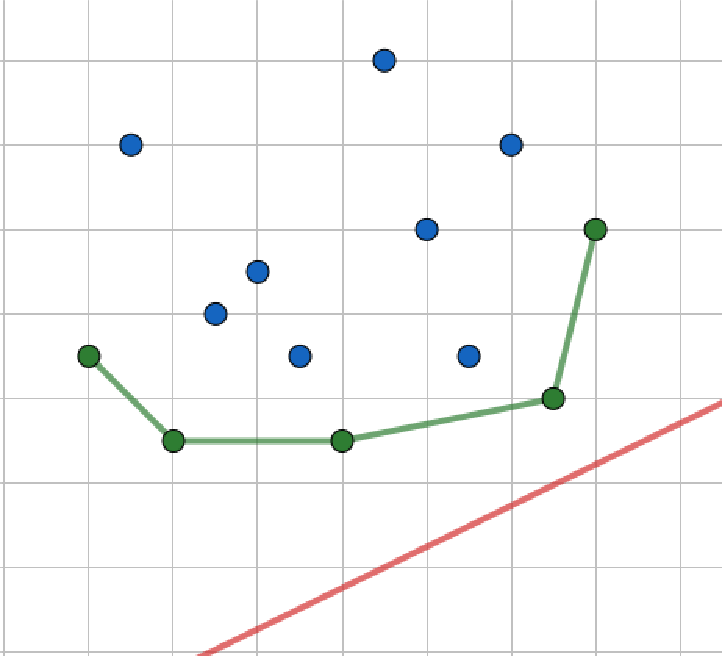
\includegraphics[width=0.5\linewidth]{fig/fig1.pdf}
	\end{framed}
	\caption{}
	\label{fig:fig1}
\end{figure}

% \begin{figure}
%   \centering
%   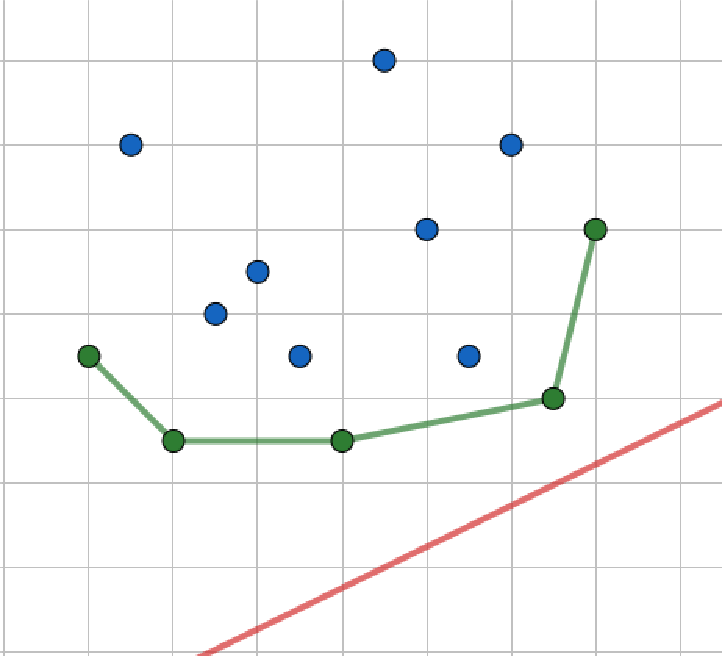
\includegraphics[width=0.6\linewidth]{fig/fig1.pdf}
% %   \caption{图表 1}
%   \label{fig:fig1}
% \end{figure}


于是可以在转移的同时维护 \((x_i,y_i)\)
构成的凸包,利用单调性二分得到时间复杂度为 \(\mathcal{O}(n\log n)\)
的算法。发现 \(k=2s_i\) 关于 \(i\)
单调递增,因此可以利用单调队列来维护得到时间复杂度为 \(\mathcal{O}(n)\)
的算法。

\subsection{代码实现}

\inputminted[frame=lines, numbers=left, fontsize=\footnotesize, tabsize=4, breaklines=true]{c++}{code/6.cpp}
% !TeX root = ../thuthesis-example.tex

\chapter{四边形不等式优化动态规划 \cite{Li}\ \cite{yao1980efficient}}

\section{四边形不等式}

若对于任意整数 \(l_1,l_2,r_2,r_1\) 满足
\(l_1\le l_2\le r_2\le r_1\),若二元函数 \(w(x,y)\) 满足 \[
w(l_1,r_1)+w(l_2,r_2)\ge w(l_1,r_2)+w(l_2,r_1)\tag{1}
\] 则称 \(w\) 满足四边形不等式。四边形不等式有一个经典的等价形式: \[
w(l,r+1)+w(l+1,r)\ge w(l,r)+w(l+1,r+1)\tag{2}
\] 其中
\(l < r\).

由(1)得到(2)较为显然,由(2)推出(1)可以通过数学归纳法证得。

假设对于 \(l+x < r\) 有 \[
w(l,r+1)+w(l+x,r)\ge w(l,r)+w(l+x,r+1)\\
\] 在 \(x=1\) 时此式为(1).

对于 \(l+x+1 < r\),根据(2)有 \[
w(l+x,r+1)+w(l+x+1,r)\ge w(l+x,r)+w(l+x+1,r+1)\\
\]

两式相加可得 \[
w(l,r+1)+w(l+x+1,r)\ge w(l,r)+w(l+x+1,r+1)
\]

同理可得 \(w(l,r+y)+w(l+x,r)\ge w(l,r)+w(l+x,r+y)\),于是得证。

\section{四边形不等式对一维 DP 的优化}

在优化一维 DP 时,DP 的形式往往为
\(f[i]=\min\limits_{0\le j < i}\{f[j]+w(j,i)\}\)。不妨用 \(d[i]\) 表示
使 \(f[i]\) 取得最小值的 \(j\),那么称 \(f\) 具有决策单调性当且仅当:
若 \(w\) 满足四边形不等式,则 \(d\)单调不减。利用此性质可以使时间复杂度为
\(\mathcal{O}(n^2)\) 的计算简化为
\(\mathcal{O}(n\log n)\)。本文将不对这类优化进行细致探讨。

\section{四边形不等式对二维 DP 的优化}

在优化二维 DP 时,DP 的形式则多为
\(f[i][j]=\min\limits_{i\le k < j}\{f[i][k]+f[k+1][j]+w(i,j)\}(i < j)\),\(f[i][i]=0\)。

不妨记 \(d[i][j]\) 为使 \(f[i][j]\)取得最小值的 \(k\),那么

\begin{itemize}

\item
  若下列命题同时成立

  \begin{enumerate}
  \def\labelenumi{\arabic{enumi}.}

  \item
    \(w\) 满足四边形不等式,
  \item
    对于任意 \(l_1\le l_2\le r_2\le r_1\),有
    \(w(l_1,r_1)\ge w(l_2,r_2)\),
  \end{enumerate}
\item
  则可推出以下命题

  \begin{enumerate}
  \def\labelenumi{\arabic{enumi}.}

  \item
    \(f\) 也满足四边形不等式,
  \item
    \(d[i][j]\le d[i+1][j]\) 且 \(d[i][j]\le d[i][j+1]\).
  \end{enumerate}
\end{itemize}

对于满足 \(d[i][j]\le \min\{d[i+1][j],d[i][j+1]\}\) 的,我们称 \(\operatorname{dp}\)
具有二维决策单调性。在对 \(f[i][j]\) 进行计算时,仅考察位于
\([d[i][j-1],d[i+1][j]]\) 中的 \(k\) 可以使时间复杂度从
\(\mathcal{O}(n^3)\) 优化为 \(\mathcal{O}(n^2)\).

\subsection{对满足四边形不等式的证明}

关于 \(f\) 满足四边形不等式的证明,考虑使用数学归纳法。

1. 当 \(r-l=1\) 时, \[
\begin{array}{c}
f[l][r+1]+f[l+1][r]=f[l][l+2]\ge w(l,l+2)\\
f[l][r]+f[l+1][r+1]=f[l][l+1]+f[l+1][l+2]=w(l,l+1)+w(l+1,l+2)\\
f[l][r+1]+f[l+1][r]\ge f[l][r]+f[l+1][r+1]
\end{array}
\]

2. 设在 \(r-l < k\) 时,\(f\) 满足四边形不等式。

为方便起见,设 \(x=d[l][r+1],y=d[l+1][r]\),那么: \[
f[l][r+1]+f[l+1][r]=(f[l][x]+f[x+1][r+1]+w(l,r+1))+(f[l+1][y]+f[y+1][r]+w(l+1,r))\\
\]
\[f[l][r]+f[l+1][r+1]\le(f[l][x]+f[x+1][r]+w(l,r))+(f[l+1][y]+f[y+1][r+1]+w(l+1,r+1))
\]

欲证: \[f[l][r+1]+f[l+1][r]\ge f[l][r]+f[l+1][r+1]
\]

只需证: \[f[x+1][r+1]+f[y+1][r]+w(l,r+1)+w(l+1,r)\ge f[x+1][r]+f[y+1][r+1]+w(l,r)+w(l+1,r+1)
\]

只需证: \[
\begin{array}{c}
f[x+1][r+1]+f[y+1][r]\ge f[x+1][r]+f[y+1][r+1]\\
w(l,r+1)+w(l+1,r)\ge w(l,r)+w(l+1,r+1)
\end{array}
\]

两式分别可以由归纳假设以及 \(w\) 满足四边形不等式得到。

综合1,2,即可证明 \(f\) 满足四边形不等式。

\subsection{对二维决策单调性的证明}

关于二维决策单调性的证明,设 \(x=d[i][j]\),\(i\le k < x\)。根据 \(f\)
满足四边形不等式和 \(d[i][j]\) 的最优性,有 \[
f[i][x]+f[i+1][k]\ge f[i][k]+f[i+1][x]\\
f[i][k]+f[k+1][j]\ge f[i][x]+f[x+1][j]
\] 可以得到 \[
f[i+1][k]+f[k+1][j]\ge f[i+1][x]+f[x+1][j]
\] 因此对于 \(f[i+1][j]\) 的转移,\(k\in [i,d[i][j])\) 一定不优于
\(d[i][j]\),有 \(d[i+1][j]\ge d[i][j]\)。
类似的,设 \(x < k\le j\),有 \[
f[x+1][j]+f[k+1][j-1]\ge f[x+1][j-1]+f[k+1][j]\\
f[i][k]+f[k+1][j]\ge f[i][x]+f[x+1][j]
\] 可以得到 \[
f[i][k]+f[k+1][j-1]\ge f[i][x]+f[x+1][j-1]
\] 即 \(d[i][j-1]\le d[i][j]\).

\subsection{对时间复杂度的证明}

关于时间复杂度是 \(\mathcal{O}(n^2)\) 的证明,考虑 \[
\begin{aligned}
&\sum_{i=1}^{n-1}\sum_{j=i+1}^n(d[i+1][j]-d[i][j-1])\\
=&\sum_{i=2}^n\sum_{j=i+1}^nd[i][j]-\sum_{i=1}^{n-1}\sum_{j=i}^{n-1}d[i][j]\\
=&\sum_{i=1}^{n-1}d[i][n]-\sum_{j=2}^nd[1][j]-\sum_{i=1}^nd[i][i]
\end{aligned}
\]
并且 \(d[i][j]\in[1,n]\),因此
\(\mathcal{O}(\sum_{i=1}^{n-1}\sum_{j=i+1}^n(d[i+1][j]-d[i][j-1]))=\mathcal{O}(n^2)\).

\section{应用实例一}

\subsection{题目描述}

有 \(n\) 堆直线排列的石子,第 \(i\) 堆石子有 \(a[i]\) 个。

规定每次只能合并任意相邻的两堆石子,并产生两堆石子数量之和的疲劳值。现在要将石子有序的合并成一堆,试求最小总疲劳值。

数据范围:\(1\le n\le 5000\).

\subsection{解题思路}

设 \(\operatorname{dp}[i][j]\) 为将下标在区间 \([i,j]\)
内的石子合并为一堆所需的最小疲劳值,\(w(i,j)=\sum_{k=i}^ja[k]\),那么有
\[
\operatorname{dp}[i][j]=
\left\{
\begin{array}{ll}
\min\limits_{i\le k < j}\{\operatorname{dp}[i][k]+\operatorname{dp}[k+1][j]+w(i,j)\},&i < j\\
0,&i=j\\
+\infty, &i>j
\end{array}
\right.
\] 直接转移时间复杂度为 \(\mathcal{O}(n^3)\),不能接受。发现 \(w\) 满足
\[
w(l,r+1)+w(l+1,r)=w(l,r)+w(l+1,r+1)
\] 即复合四边形不等式条件,因此可以对上述 DP 进行优化,达到
\(\mathcal{O}(n^2)\) 的时间复杂度。

\subsection{代码实现}

\inputminted[frame=lines, numbers=left, fontsize=\scriptsize, tabsize=4, breaklines=true]{c++}{code/7.cpp}

\section{应用实例二}

\subsection{题目来源}

题目名称:邮局。

题目选自:IOI2000.

\subsection{题目描述}

给定 \(n\) 个村庄在一条直线上的坐标。现在要选一些村庄建立 \(k\)
个邮局,使得每个村庄与其最近的邮局之间的距离总和最小。试求这个最小距离和。

数据范围:用 \(p_i\) 表示村庄坐标,则
\(1\le k\le 300\),\(k\le n\le 3000\),\(1 \le p_i\le 10000\).

\subsection{解题思路}

首先将村庄按其在坐标轴上的位置排序,设第 \(i\) 个村庄的坐标为 \(x_i\)。

设 \(\operatorname{dp}[i][j]\) 表示前 \(i\) 个村庄建立 \(j\)
个邮局的最小距离和,\(w(l,r)\) 表示在第 \(p\) 个村庄建立一个邮局所得到的
\(\sum_{i=l}^r|x_i-x_p|\) 的最小值。不难看出
\(p=\lfloor \frac{l+r}{2}\rfloor\),因此 \[
\begin{aligned}
w(l,r)&=(\sum_{i=p+1}^rx_i-x_p(r-p))+(x_p(p-l)-\sum_{i=l}^{p-1}x_i)\\
w(l,r)&=w(l,r-1)+x_r-x_p\\
w(l,r)&=w(l+1,r)+x_p-x_l\\
\end{aligned}
\] 可以在 DP 转移前 \(\mathcal{O}(n^2)\)
递推,也可以使用前缀和每次转移时 \(\mathcal{O}(1)\) 计算。

同时 DP 递推式有 \[
\operatorname{dp}[i][j]=
\left\{
\begin{array}{ll}
\min\limits_{1\le k\le i}\{\operatorname{dp}[k-1][j-1]+w(k,i)\},&\text{if } i\neq0,j\neq0\\
1,&\text{if }i=0 j=0\\
0,&\text{otherwise}
\end{array}
\right.
\] 直接递推是 \(\mathcal{O}(n^2k)\) 的,不能接受。发现 \[
\begin{aligned}
w(l,r)+w(l+1,r-1)&=2w(l+1,r-1)+x_r-x_l\\
w(l+1,r)+w(l,r-1)&=2w(l+1,r-1)+x_r-x_l-(x_{\lfloor \frac{l+r+1}{2}\rfloor}-x_{\lfloor \frac{l+r-1}{2}\rfloor})
\end{aligned}
\] 因为 \(x\) 递增,有
\((x_{\lfloor \frac{l+r+1}{2}\rfloor}-x_{\lfloor \frac{l+r-1}{2}\rfloor})\ge0\),所以
\(w(l,r)+w(l+1,r-1)\ge w(l+1,r)+w(l,r-1)\),\(w\)
满足四边形不等式,\(\operatorname{dp}\)
满足四边形不等式。因此对转移时计算的区间进行优化就能达到
\(\mathcal{O}(nk)\) 的时间复杂度。

\subsection{代码实现}

\inputminted[frame=lines, numbers=left, fontsize=\scriptsize, tabsize=4, breaklines=true]{c++}{code/8.cpp}

% !TeX root = ../thuthesis-example.tex

\chapter{CDQ 分治优化 DP}

\section{CDQ 分治}

CDQ
分治最早为陈丹琦在《从\textless cash\textgreater 谈一类分治算法的应用》中整理的,因此以
CDQ 命名。

陈丹琦本人整理的 CDQ
分治应用方法主要为先将在线维护的问题转换为离线问题,并添加一个操作时间的维度,再对高维的偏序问题进行分治处理。后来引申的
CDQ
分治应用范围则包括了可离线的高维偏序问题以及转移包括高维偏序条件的动态规划问题。

下文将探讨 CDQ 分治对转移包括高维偏序条件的动态规划问题的优化。

\section{应用实例一}

\subsection{题目描述}

给定一个长度为 \(n\) 的排列
\(a\),其中有若干位置上的数字已经确定了,剩下位置上的数字不确定。

你需要钦定未被确定的位置上的数字,使得得到的排列的最长上升子序列(LIS,Longest
Increasing Subsequence)长度尽量长。试求出这个最长长度。

数据范围:\(n\leq 10^5\).

\subsection{解题思路}

注意到 ``是一个排列''
这个限制,事实上仅仅限制了那些未被确定的位置上的数字不能与已经确定的位置相同,而我们在计算最优答案时并不需要特别处理未被确定的数字之间是否相同,因为
LIS 中不能出现两个相同的数字,因此剩下位置上出现相同数字一定不优。

设 \(f(i,j)\) 表示对于 \(a\) 数组长度为 \(i\)
的前缀,在所有钦定方案中,以 \(j\) 结尾的最长的 LIS 长度。有转移:

\begin{itemize}
\item
  若位置 \(i\) 被确定了,则
  \(f(i,x)=\begin{cases}\max_{j < p_i}(f(i-1,j))+1&x=p_i\\0&x\not=p_i\end{cases}\);
\item
  否则 \(f(i,j)=\max\{\max_{k < j}(f(i-1,k))+1,f(i-1,j)\}\),这里的
  \(j\) 必须不在已经确定的数字中出现过。
\end{itemize}

这样直接转移是 \(\mathcal{O}(n^2)\) 的。

但是二维 dp 是不方便使用 CDQ 分治优化的,仍然考虑转成一维 dp 的形式。

设 \(f(i)\) 表示以位置 \(i\) 结尾的最长 LIS,此处位置 \(i\)
的数字必须被确定了。

则枚举 LIS 中上一个有确定数字的位置。用 \(\operatorname{cnt}[i]\) 表示
\(a\) 长度为 \(i\)
的前缀中没被确定的位置个数,\(\operatorname{rem}[p_i]\) 表示 \(< p_i\)
且未出现在被确定的位置的数字个数,可以得到: \[
f(i)=\max_{p_j < p_i}\{f(j)+\min\{\operatorname{cnt}[i]-\operatorname{cnt}[j],\operatorname{rem}[p_i]-\operatorname{rem}[p_j]\}\}+1
\] 注意到这里同时有 \(p_j<p_i\) 和 \(j<i\) 两个限制,且中间的 \(\min\)
可以分类讨论为两种情况:

\begin{enumerate}
\def\labelenumi{\arabic{enumi}.}

\item
  \(\operatorname{cnt}[i]-\operatorname{cnt}[j]\geq\operatorname{rem}[p_i]-\operatorname{rem}[p_j] \iff \operatorname{cnt}[i]-\operatorname{rem}[p_i]\geq\operatorname{cnt}[j]-\operatorname{rem}[p_j]\)
\item
  \(cnt[i]-cnt[j]<\operatorname{rem}[p_i]-\operatorname{rem}[p_j] \iff cnt[i]-\operatorname{rem}[p_i]<cnt[j]-\operatorname{rem}[p_j]\)
\end{enumerate}

这也就相当于第三个限制,加上前两个就是三维偏序。因此我们先按下标分治,然后左右两边分别按
\(\operatorname{cnt}[i]-\operatorname{rem}[p_i]\)
排序,以第一种情况为例,双指针扫的时候用树状数组维护
\(f(j)-\operatorname{rem}[p_j]\) 即可。

整体时间复杂度 \(\mathcal{O}(n \log^2 n)\),空间复杂度
\(\mathcal{O}(n)\)。

\subsection{代码实现}

\inputminted[frame=lines, numbers=left, fontsize=\footnotesize, tabsize=4, breaklines=true]{c++}{code/9.cpp}

\section{应用实例二}

\subsection{题目来源}

题目名称:Building Bridges.

题目选自:CEOI2017.

\subsection{题目描述}

给定 \(n\) 个柱子,每个柱子用 \((h_i,w_i)\) 描述。拆除第 \(i\)
根柱子的代价为 \(w_i\)。在 \(i,j\) 之间架桥的代价为
\((h_i-h_j)^2\),同时还需要拆除 \([i+1,j-1]\)
之间的所有柱子。求通过桥梁把 \(1\) 和 \(n\) 连通的最小代价。

数据范围:\(2\leq n\leq 10^5\),\(0\leq h_i,|w_i|\leq 10^6\).

\subsection{解题思路}

不妨设 \(\operatorname{dp}[i]\) 为通过桥梁将 \(1\) 和 \(i\)
联通的最小代价,\(s_i=\sum_{i\in[1,i]}w_i\),不难得到 \[
\operatorname{dp}[i]=\min_{j < i}(dp[j]+s_{i-1}-s_j+(h_i-h_j)^2)
\] 将 \(\min\) 去掉可以得到 \[
(\operatorname{dp}[j]-s_j+h_j^2)=h_i\times(2h_j)-(s_{i-1}+h_i^2)+\operatorname{dp}[i]
\]

发现能斜率优化,然而直接进行斜率优化需要满足斜率 \(2h_j\) 单调,因此考虑
CDQ 分治。具体来讲,以第一维为下标,计算 \(\operatorname{cdq}(l,r)\)
时,令 \(\operatorname{mid}=\lfloor\frac{l+r}{2}\rfloor\),对
\([l,\operatorname{mid}]\) 中的下标 \(i\) 直接计算出由
\((\operatorname{dp}[i]-s_i+h_i^2,h_i)\) 构成的下凸包
,\([\operatorname{mid}+1,r]\) 中的元素按照 \(h\) 排序然后做斜率优化 DP
计算贡献即可。

\subsection{代码实现}

\inputminted[frame=lines, numbers=left, fontsize=\footnotesize, tabsize=4, breaklines=true]{c++}{code/10.cpp}
% !TeX root = ../thuthesis-example.tex

\chapter{结语}

在解决动态规划问题时,人们常常会受算法难度和思路的限制。经过此次学习,本组详细整理并掌握了两种复杂的动态规划算法以及四种可以被广泛应用的算法优化方式,形成文字化资料,可以被后人利用。而其中本组所附上的典例解析可以作为参考资料,有利于后人对于该算法的学习,可以更好地理解并应用该算法。

通过本次课题研究,我们对文献法的掌握更加深入。本组在后续的成文过程中也参考了各资料的成文方式,使我们的文章深入浅出,更为简洁易懂。本小组成员各司其职,分工合理。这使得我们的研学速度快,成果质量高。我们的心态也逐渐变得稳健,铸就了迎难而上,不放弃的精神。

本次研学我们的创新意识稍有不足,主要进行了资料的整合而非独立,全新的创作。以后需加以改进。


% 其他部分
\backmatter

% 参考文献
\bibliography{ref/refs}  % 参考文献使用 BibTeX 编译
% \printbibliography       % 参考文献使用 BibLaTeX 编译

% 附录
% 本科生需要将附录放到声明之后,个人简历之前
\appendix
% % % !TeX root = ../thuthesis-example.tex

% \begin{survey}
% \label{cha:survey}

% \title{Title of the Survey}
% \maketitle


% \tableofcontents


% 本科生的外文资料调研阅读报告。


% \section{Figures and Tables}

% \subsection{Figures}

% An example figure in appendix (Figure~\ref{fig:appendix-survey-figure}).

% \begin{figure}
%   \centering
%   
\includegraphics[width=0.6\linewidth]{example-image-a.pdf}
%   \caption{Example figure in appendix}
%   \label{fig:appendix-survey-figure}
% \end{figure}


% \subsection{Tables}

% An example table in appendix (Table~\ref{tab:appendix-survey-table}).

% \begin{table}
%   \centering
%   \caption{Example table in appendix}
%   \begin{tabular}{ll}
%     \toprule
%     File name       & Description                                         \\
%     \midrule
%     thuthesis.dtx   & The source file including documentaion and comments \\
%     thuthesis.cls   & The template file                                   \\
%     thuthesis-*.bst & BibTeX styles                                       \\
%     thuthesis-*.bbx & BibLaTeX styles for bibliographies                  \\
%     thuthesis-*.cbx & BibLaTeX styles for citations                       \\
%     \bottomrule
%   \end{tabular}
%   \label{tab:appendix-survey-table}
% \end{table}


% \section{Equations}

% An example equation in appendix (Equation~\eqref{eq:appendix-survey-equation}).
% \begin{equation}
%   \frac{1}{2 \uppi \symup{i}} \int_\gamma f = \sum_{k=1}^m n(\gamma; a_k) \mathscr{R}(f; a_k)
%   \label{eq:appendix-survey-equation}
% \end{equation}


% \section{Citations}

% Example citations in appendix.
% \cite{abrahams99tex}
% \cite{salomon1995advanced}
% \cite{abrahams99tex,salomon1995advanced}


% \bibliographystyle{unsrtnat}
% \bibliography{ref/appendix}

% \end{survey}
       % 本科生:外文资料的调研阅读报告
% % !TeX root = ../thuthesis-example.tex

\begin{translation}
\label{cha:translation}

\title{书面翻译题目}
\maketitle

\tableofcontents


本科生的外文资料书面翻译。


\section{图表示例}

\subsection{图}

附录中的图片示例(图~\ref{fig:appendix-translation-figure})。

\begin{figure}
  \centering
  
\includegraphics[width=0.6\linewidth]{example-image-a.pdf}
  \caption{附录中的图片示例}
  \label{fig:appendix-translation-figure}
\end{figure}


\subsection{表格}

附录中的表格示例(表~\ref{tab:appendix-translation-table})。

\begin{table}
  \centering
  \caption{附录中的表格示例}
  \begin{tabular}{ll}
    \toprule
    文件名          & 描述                         \\
    \midrule
    thuthesis.dtx   & 模板的源文件,包括文档和注释 \\
    thuthesis.cls   & 模板文件                     \\
    thuthesis-*.bst & BibTeX 参考文献表样式文件    \\
    thuthesis-*.bbx & BibLaTeX 参考文献表样式文件  \\
    thuthesis-*.cbx & BibLaTeX 引用样式文件        \\
    \bottomrule
  \end{tabular}
  \label{tab:appendix-translation-table}
\end{table}


\section{数学公式}

附录中的数学公式示例(公式\eqref{eq:appendix-translation-equation})。
\begin{equation}
  \frac{1}{2 \uppi \symup{i}} \int_\gamma f = \sum_{k=1}^m n(\gamma; a_k) \mathscr{R}(f; a_k)
  \label{eq:appendix-translation-equation}
\end{equation}


\section{文献引用}

文献引用示例\cite{abrahams99tex}。


\appendix

\section{附录}

附录的内容。


% 书面翻译的参考文献
\bibliographystyle{unsrtnat}
\bibliography{ref/appendix}

% 书面翻译对应的原文索引
\begin{translation-index}
  \nocite{salomon1995advanced}
  \bibliographystyle{unsrtnat}
  \bibliography{ref/appendix}
\end{translation-index}

\end{translation}
  % 本科生:外文资料的书面翻译
% % !TeX root = ../thuthesis-example.tex

\chapter{补充内容}

附录是与论文内容密切相关、但编入正文又影响整篇论文编排的条理和逻辑性的资料,例如某些重要的数据表格、计算程序、统计表等,是论文主体的补充内容,可根据需要设置。


\section{图表示例}

\subsection{图}

附录中的图片示例(图~\ref{fig:appendix-figure})。

\begin{figure}
  \centering
  
\includegraphics[width=0.6\linewidth]{example-image-a.pdf}
  \caption{附录中的图片示例}
  \label{fig:appendix-figure}
\end{figure}


\subsection{表格}

附录中的表格示例(表~\ref{tab:appendix-table})。

\begin{table}
  \centering
  \caption{附录中的表格示例}
  \begin{tabular}{ll}
    \toprule
    文件名          & 描述                         \\
    \midrule
    thuthesis.dtx   & 模板的源文件,包括文档和注释 \\
    thuthesis.cls   & 模板文件                     \\
    thuthesis-*.bst & BibTeX 参考文献表样式文件    \\
    thuthesis-*.bbx & BibLaTeX 参考文献表样式文件  \\
    thuthesis-*.cbx & BibLaTeX 引用样式文件        \\
    \bottomrule
  \end{tabular}
  \label{tab:appendix-table}
\end{table}


\section{数学公式}

附录中的数学公式示例(公式\eqref{eq:appendix-equation})。
\begin{equation}
  \frac{1}{2 \uppi \symup{i}} \int_\gamma f = \sum_{k=1}^m n(\gamma; a_k) \mathscr{R}(f; a_k)
  \label{eq:appendix-equation}
\end{equation}


% 致谢
% % % !TeX root = ../thuthesis-example.tex

% \begin{acknowledgements}
%   衷心感谢导师×××教授和物理系××副教授对本人的精心指导。他们的言传身教将使我终生受益。

%   在美国麻省理工学院化学系进行九个月的合作研究期间,承蒙 Robert Field 教授热心指导与帮助,不胜感激。

%   感谢×××××实验室主任×××教授,以及实验室全体老师和同窗们学的热情帮助和支持!

%   本课题承蒙国家自然科学基金资助,特此致谢。
% \end{acknowledgements}


% 声明
% \statement
% 将签字扫描后的声明文件 scan-statement.pdf 替换原始页面
% \statement[file=scan-statement.pdf]
% 本科生编译生成的声明页默认不加页脚,插入扫描版时再补上;
% 研究生编译生成时有页眉页脚,插入扫描版时不再重复。
% 也可以手动控制是否加页眉页脚
% \statement[page-style=empty]
% \statement[file=scan-statement.pdf, page-style=plain]

% 个人简历、在学期间完成的相关学术成果
% 本科生可以附个人简历,也可以不附个人简历
% % !TeX root = ../thuthesis-example.tex

\begin{resume}

  \section*{个人简历}

  197× 年 ×× 月 ×× 日出生于四川××县。

  1992 年 9 月考入××大学化学系××化学专业,1996 年 7 月本科毕业并获得理学学士学位。

  1996 年 9 月免试进入清华大学化学系攻读××化学博士至今。


  \section*{在学期间完成的相关学术成果}

  \subsection*{学术论文}

  \begin{achievements}
    \item Yang Y, Ren T L, Zhang L T, et al. Miniature microphone with silicon-based ferroelectric thin films[J]. Integrated Ferroelectrics, 2003, 52:229-235.
    \item 杨轶, 张宁欣, 任天令, 等. 硅基铁电微声学器件中薄膜残余应力的研究[J]. 中国机械工程, 2005, 16(14):1289-1291.
    \item 杨轶, 张宁欣, 任天令, 等. 集成铁电器件中的关键工艺研究[J]. 仪器仪表学报, 2003, 24(S4):192-193.
    \item Yang Y, Ren T L, Zhu Y P, et al. PMUTs for handwriting recognition. In press[J]. (已被Integrated Ferroelectrics录用)
  \end{achievements}


  \subsection*{专利}

  \begin{achievements}
    \item 任天令, 杨轶, 朱一平, 等. 硅基铁电微声学传感器畴极化区域控制和电极连接的方法: 中国, CN1602118A[P]. 2005-03-30.
    \item Ren T L, Yang Y, Zhu Y P, et al. Piezoelectric micro acoustic sensor based on ferroelectric materials: USA, No.11/215, 102[P]. (美国发明专利申请号.)
  \end{achievements}

\end{resume}


% 指导教师/指导小组学术评语
% 本科生不需要
% % !TeX root = ../thuthesis-example.tex

\begin{comments}
% \begin{comments}[name = {指导小组学术评语}]
% \begin{comments}[name = {Comments from Thesis Supervisor}]
% \begin{comments}[name = {Comments from Thesis Supervision Committee}]

  论文提出了……

\end{comments}


% 答辩委员会决议书
% 本科生不需要
% % !TeX root = ../thuthesis-example.tex

\begin{resolution}

  论文提出了……

  论文取得的主要创新性成果包括:

  1. ……

  2. ……

  3. ……

  论文工作表明作者在×××××具有×××××知识,具有××××能力,论文××××,答辩××××。

  答辩委员会表决,(×票/一致)同意通过论文答辩,并建议授予×××(姓名)×××(门类)学博士/硕士学位。

\end{resolution}


% 本科生的综合论文训练记录表(扫描版)
% \record{file=scan-record.pdf}

\end{document}
